\chapter{分治法}


\section{Pow(x,n)} %%%%%%%%%%%%%%%%%%%%%%%%%%%%%%
\label{sec:pow}


\subsubsection{描述}
Implement pow(x, n).


\subsubsection{分析}
二分法,$x^n = x^{n/2} \times x^{n/2} \times x^{n\%2}$


\subsubsection{代碼}
\begin{Code}
//LeetCode, Pow(x, n)
// 二分法,$x^n = x^{n/2} * x^{n/2} * x^{n\%2}$
// 時間複雜度O(logn),空間複雜度O(1)
class Solution {
public:
    double myPow(double x, int n) {
        long long nn = n // 使用 64 bit 來處理 INT_MIN 由負變正 case
        if (nn < 0) return 1.0 / power(x, -nn);
        else return power(x, nn);
    }
private:
    double power(double x, long long nn) {
        if (nn == 0) return 1;
        double v = power(x, nn / 2);
        if (nn % 2 == 0) return v * v;
        else return v * v * x;
    }
};
\end{Code}


\subsubsection{相關題目}

\begindot
\item Sqrt(x),見 \S \ref{sec:sqrt}
\myenddot


\section{Sqrt(x)} %%%%%%%%%%%%%%%%%%%%%%%%%%%%%%
\label{sec:sqrt}

\subsubsection{描述}
Implement int \fn{sqrt(int x)}.

Compute and return the square root of \fn{x}.


\subsubsection{分析}
二分查找


\subsubsection{代碼}
\begin{Code}
// LeetCode, Sqrt(x)
// 二分查找
// 時間複雜度O(logn),空間複雜度O(1)
class Solution {
public:
    int mySqrt(int x) {
        int left = 1, right = x / 2;
        int last_mid;  // 記錄最近一次mid

        if (x < 2) return x;

        while(left <= right) {
            const int mid = left + (right - left) / 2;
            if(x / mid > mid) { // 不要用 x > mid * mid,會溢出
                left = mid + 1;
                last_mid = mid;
            } else if(x / mid < mid) {
                right = mid - 1;
            } else {
                return mid;
            }
        }
        return last_mid;
    }
};
\end{Code}


\subsubsection{相關題目}
\begindot
\item Pow(x),見 \S \ref{sec:pow}
\myenddot

\section{The Skyline Problem}
\label{sec:the-skyline-problem}

\subsubsection{描述}
A city's skyline is the outer contour of the silhouette formed by all the buildings in that city when viewed from a distance. Now suppose you are given the locations and height of all the buildings as shown on a cityscape photo (Figure A), write a program to output the skyline formed by these buildings collectively (Figure B).

\begin{center}
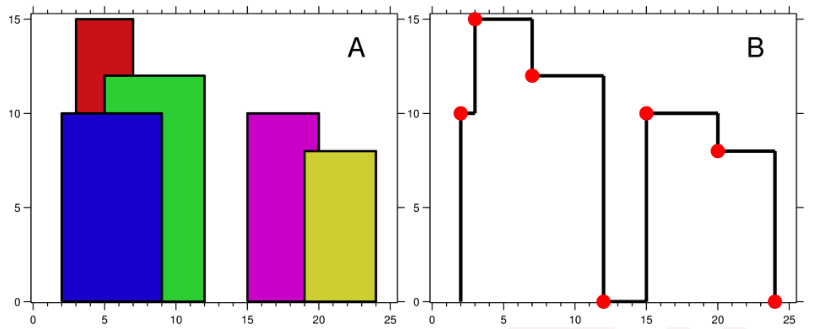
\includegraphics[width=250pt]{the-skyline-problem.png}\\
\figcaption{Skyline Problem}\label{fig:the-skyline-problem}
\end{center}

The geometric information of each building is represented by a triplet of integers [Li, Ri, Hi], where Li and Ri are the x coordinates of the left and right edge of the ith building, respectively, and Hi is its height. It is guaranteed that 0 ≤ Li, Ri ≤ INT_MAX, 0 < Hi ≤ INT_MAX, and Ri - Li > 0. You may assume all buildings are perfect rectangles grounded on an absolutely flat surface at height 0.

For instance, the dimensions of all buildings in Figure A are recorded as: [ [2 9 10], [3 7 15], [5 12 12], [15 20 10], [19 24 8] ] .

The output is a list of "key points" (red dots in Figure B) in the format of [ [x1,y1], [x2, y2], [x3, y3], ... ] that uniquely defines a skyline. A key point is the left endpoint of a horizontal line segment. Note that the last key point, where the rightmost building ends, is merely used to mark the termination of the skyline, and always has zero height. Also, the ground in between any two adjacent buildings should be considered part of the skyline contour.

For instance, the skyline in Figure B should be represented as:[ [2 10], [3 15], [7 12], [12 0], [15 10], [20 8], [24, 0] ].



Notes:

\begin{enumerate}
\item The number of buildings in any input list is guaranteed to be in the range [0, 10000].
\item The input list is already sorted in ascending order by the left x position Li.
\item The output list must be sorted by the x position.
\item There must be no consecutive horizontal lines of equal height in the output skyline. For instance, [...[2 3], [4 5], [7 5], [11 5], [12 7]...] is not acceptable; the three lines of height 5 should be merged into one in the final output as such: [...[2 3], [4 5], [12 7], ...]
\end{enumerate}

\subsubsection{分析}
Nil

\subsubsection{分治法}
\begin{Code}
// 時間複雜度O(nlogn),空間複雜度O(n)
class Solution {
public:
    vector<vector<int>> getSkyline(vector<vector<int>>& buildings) {
        return DFS(buildings, 0, buildings.size());
    }
private:
    vector<vector<int>> DFS(vector<vector<int>>& buildings, int start, int end)
    {
        if (start == end)
        {
            return vector<vector<int>>();
        }
        else if (end - start == 1)
        {
            vector<vector<int>> result;
            int& startX = buildings[start][0];
            int& startY = buildings[start][2];
            int& endX = buildings[start][1];
            result.push_back({startX, startY});
            result.push_back({endX, 0});

            return result;
        }

        int mid = start + (end - start) / 2;
        auto left = DFS(buildings, start, mid);
        auto right = DFS(buildings, mid, end);

        return mergeSkylines(left, right);
    }
    vector<vector<int>> mergeSkylines(const vector<vector<int>>& left
                                      , const vector<vector<int>>& right)
    {
        int lN = left.size();
        int rN = right.size();
        int lp, rp, curP;
        int ly, ry, curY;
        int x, maxY;
        vector<vector<int>> output; output.reserve(lN + rN);
        lp = rp = curP = 0;
        ly = ry = curY = 0;
        x = maxY = 0;

        while (lp < lN && rp < rN)
        {
            if (left[lp][0] < right[rp][0])
            {
                x = left[lp][0];
                ly = left[lp][1];
                lp++;
            }
            else
            {
                x = right[rp][0];
                ry = right[rp][1];
                rp++;
            }

            maxY = max(ly, ry);

            if (curY != maxY)
            {
                UpdateOutput(output, x, maxY);
                curY = maxY;
            }
        }

        if (lp < lN)
            AppendSkylines(output, left, lp, lN, curY);
        else
            AppendSkylines(output, right, rp, rN, curY);


        return output;
    }
    void UpdateOutput(vector<vector<int>>& output, int x, int y)
    {
        if (output.empty() || output.back()[0] != x)
            output.push_back({x, y});
        else
            output.back()[1] = y;
    }
    void AppendSkylines(vector<vector<int>>& output
                        , const vector<vector<int>>& skyline, int p, int N, int curY)
    {
        while (p < N)
        {
            const int& x = skyline[p][0];
            const int& y = skyline[p][1];
            p++;

            if (curY != y)
            {
                UpdateOutput(output, x, y);
                curY = y;
            }
        }
    }
};
\end{Code}

